\section{Lebesgueova míra}\label{sec:lebesgueova-mira}

Jednimi z nejznámějších průkopníků v oblasti teorie míry byli francouzský matematik \name{Camille Jordan} (1832--1922) a italský matematik \name{Giuseppe Peano} (1958--1932), kteří ve svých publikacích popsali způsob měření "velikosti" množin, který je dnes známý jako tzv. \emph{Jordanova-Peanova míra}. Rovinu $\R^2$ si rozdělíme na čtvercovou síť, přičemž $S$ bude představovat součet obsahů všech čtverců síťě, které jsou obsaženy ve vnitřku množiny $M$ a $S^\prime$ je součeet obsahů všech čtverců sítě, které mají společný alespoň jeden bod s hranicí množiny $M$. Součet $S+S^\prime$ pak představuje obsah všech čtverců sítě, které obsahují body uzávěru množiny $M$. (Viz obrázek \ref{fig:jordan-peano-mira}.)
\begin{figure}[h]
    \centering
    \begin{subfigure}{0.4\textwidth}
        \centering
        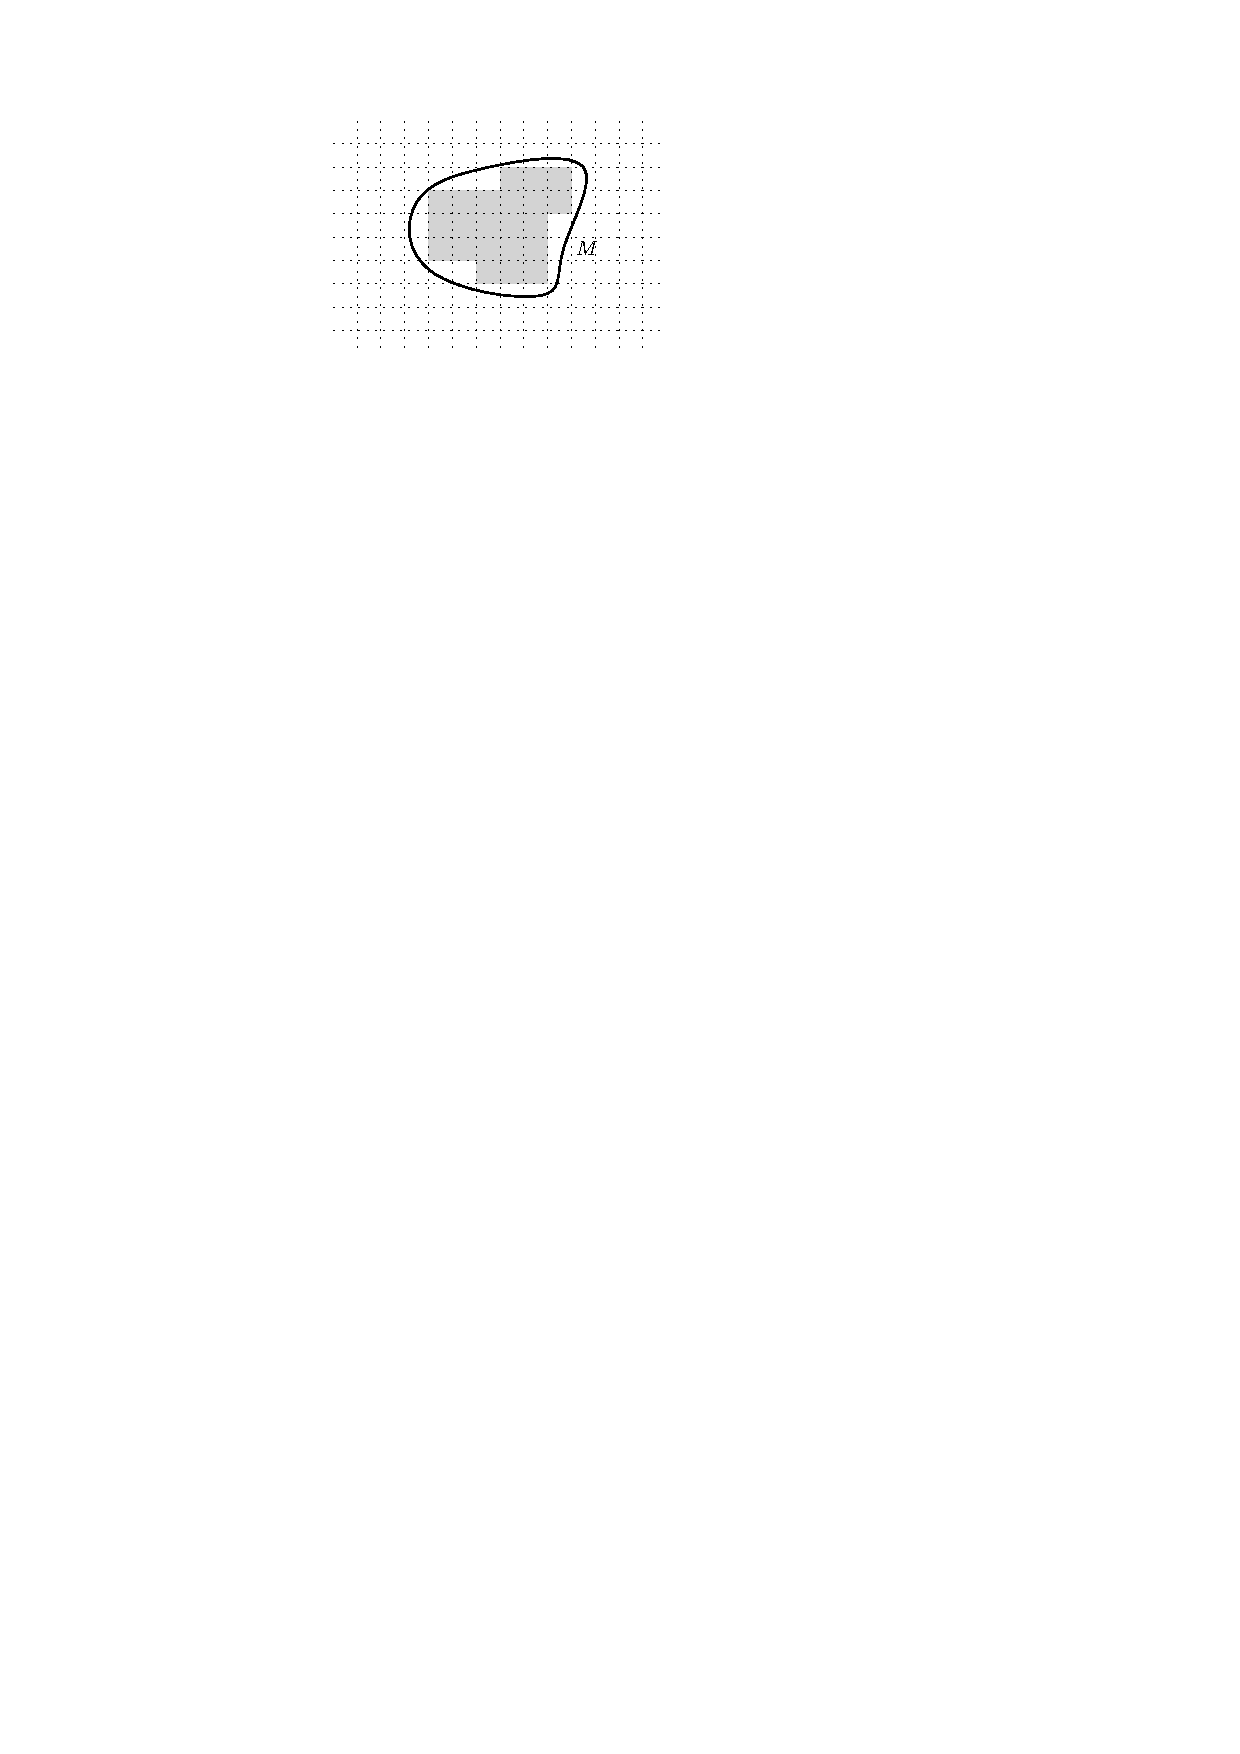
\includegraphics{ch02-jordan-peano-vnitrni-mira.pdf}
        \caption{Součet $S$}
    \end{subfigure}
    \qquad
    \begin{subfigure}{0.4\textwidth}
        \centering
        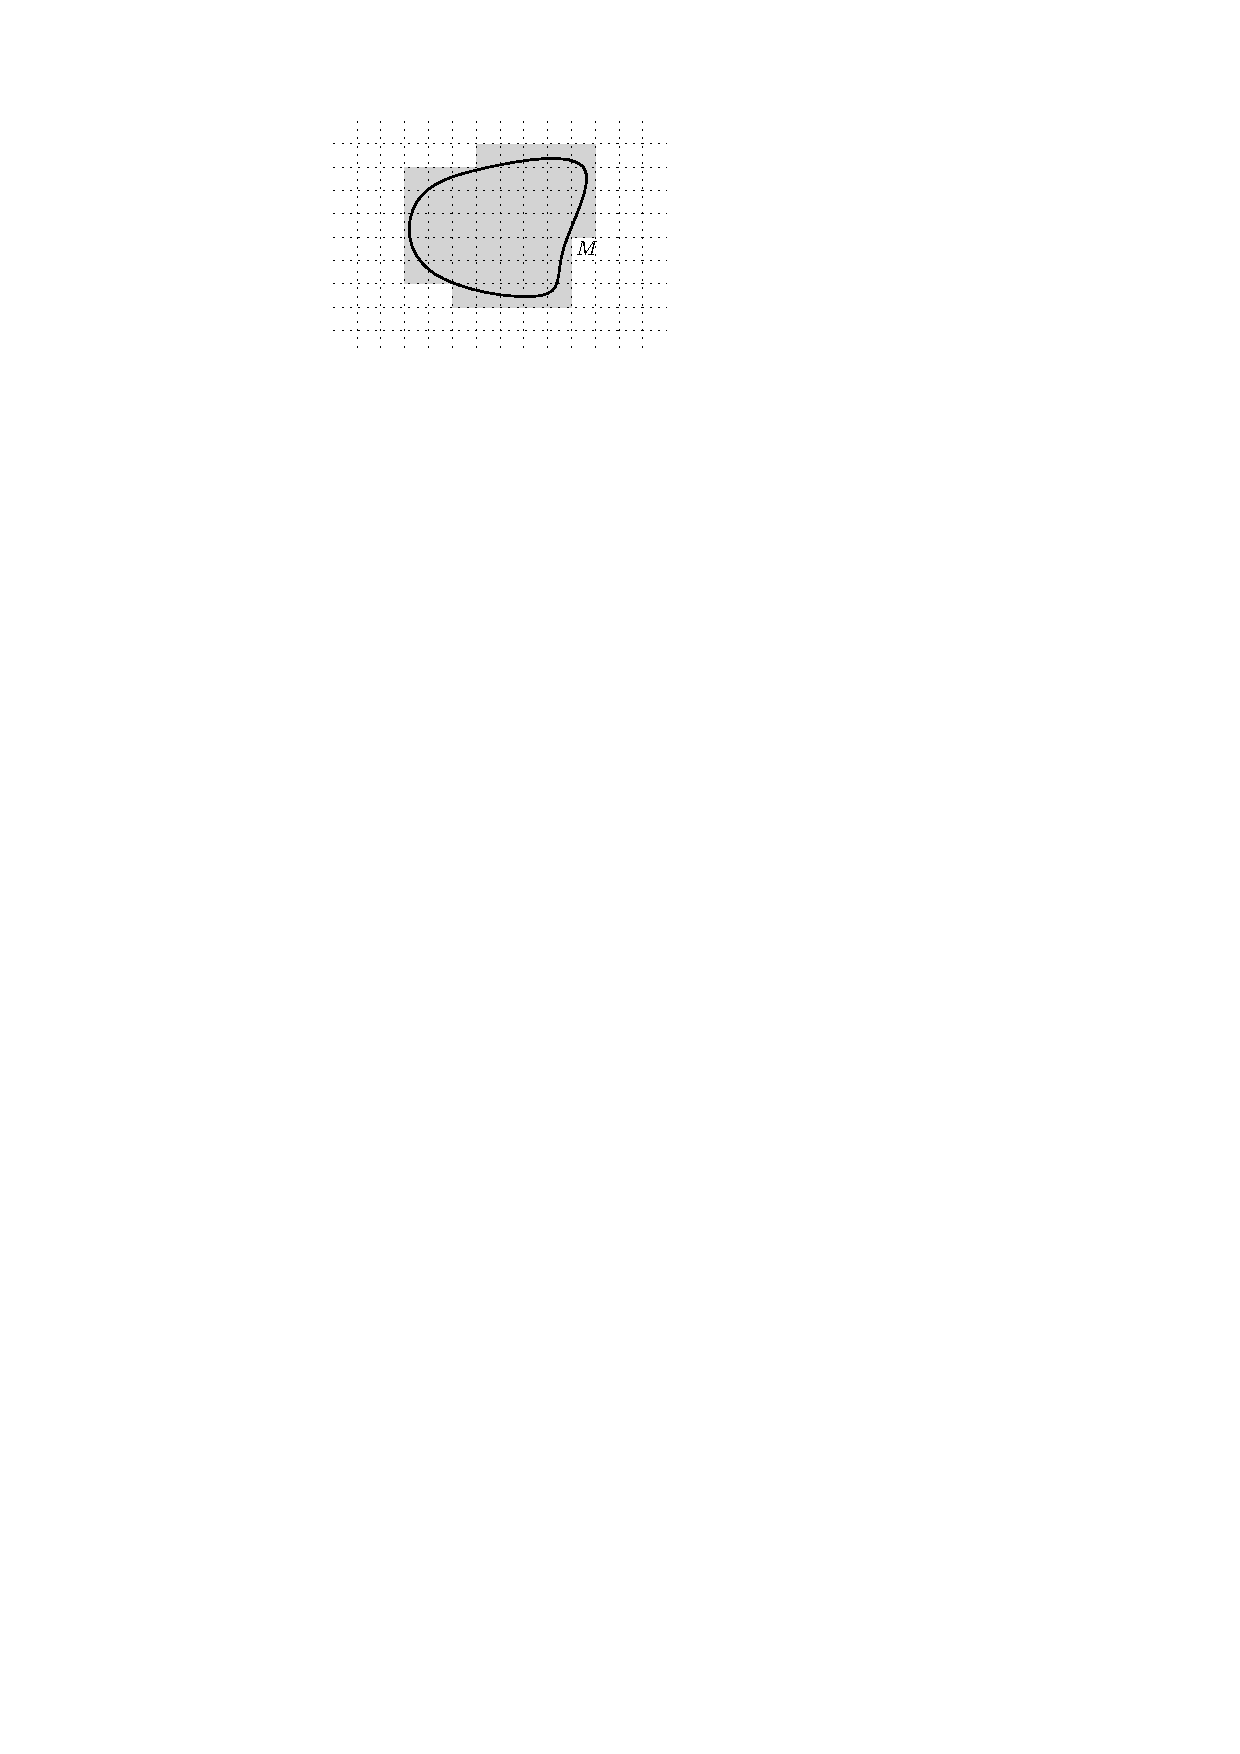
\includegraphics{ch02-jordan-peano-vnejsi-mira.pdf}
        \caption{Součet $S+S^\prime$}
    \end{subfigure}
    \caption{Vnitřní a vnější Jordanova-Peanova míra množiny $M$.}
    \label{fig:jordan-peano-mira}
\end{figure}
Při zjemňování čtvercové sítě konvergují součty $S$ a $S+S^\prime$ k limitám, které po řadě nazýváme \emph{vnitřní} a \emph{vnější Jordanova-Peanova míra}. Tato úvaha předložila základní předpoklady právě pro vznik teorie míry. \cite{Sarmanova1996}

V předešlé sekci \ref{sec:prostory-s-mirou} jsme si povídali o~pojmu \emph{míra} obecně a~podívali jsme se na několik příkladů. Obecnou ideu měření "velikosti" lze založit např. na aproximaci obecné množiny pomocí \emph{spočetných sjednocení útvarů},~jejichž "velikost" umíme jednoduše určit. V~dalším textu se omezíme pouze na množinu $\R^n$.

Na zmíněné myšlence je postavena definice tzv. \emph{$n$-rozměrné Lebesgueovy míry},~kdy obecnou množinu budeme pokrývat pomocí \emph{kvádrů}. Připomeňme,~že obecně\linebreak\mbox{$n$-rozměrným} kvádrem\index{$n$-rozměrný kvádr} $I$ rozumíme kartézský součin \emph{intervalů}
\[\langle a_1,b_1\rangle,\ldots,\langle a_n,b_n\rangle\subseteq\R,\]
tj.
\[I=\prod_{i=1}^{n}\langle a_i,b_i\rangle=\langle a_1,b_1\rangle\times\langle a_2,b_2\rangle\times\dots\times\langle a_n,b_n\rangle\]
a jeho objem\index{kvádr!objem kvádru} definujeme jako
\[\vol_n(I)=\prod_{i=1}^{n}(b_i-a_i).\]
Lze nejspíše ihned vidět,~že objem kvádru $\vol_n(I)$ je \emph{aditivní} i~\textit{subaditivní}.

Nyní si definujeme tzv. \emph{vnější Lebesgueovu míru}.
\begin{definition}[Vnější Lebesgueova míra]\label{def:vnejsi-lebegueova-mira}
    Nechť $A\subseteq\R^n$. Pak vnější $n$-rozměr\-nou Lebesgueovou mírou\index{vnější $n$-rozměrná Lebesgueova míra} $A$ je
    \[\lambda_n^*(A)=\inf\set{\sum_{j=1}^{\infty}\vol_n(I_j)\;\middle|\;\text{$I_j$ je kvádr}\;,\;A\subseteq\bigcup_{i=1}^\infty I_j}.\]
\end{definition}
Vnější Lebesgueova míra množiny intuitivně zachycuje informaci o~"velikosti" dané množiny.  Lze ihned vidět,~že pro libovolnou množinu $A\subseteq\R^n$ je $\lambda_n^*(A)\in\R_0^+$,~protože $\vol_n(I_j)\geqslant0$ pro každé $j\in\N$.
\begin{example}\label{ex:lebegueova-mira-trivialni-priklady}
    Ukažme si některé triviální příklady výpočtů vnější Lebesgueovy míry z definice (viz \ref{def:vnejsi-lebegueova-mira}),~tedy budeme hledat příslušné pokrytí dané množiny.
    \begin{itemize}
        \item Pro prázdnou množinu $\emptyset$ je $\lambda_n^*(\emptyset)=0$,~neboť $\emptyset\subseteq\prod_{i=1}^{n}\langle0,0\rangle$ (prázdnou množinu lze pokrýt jakýmkoliv kvádrem nulového objemu) a
        \[\vol_n\left(\prod_{i=1}^{n}\langle0,0\rangle\right)=0.\]
        \item Mějme libovolnou konečnou množinu $A=\set{x_1,x_2,\dots,x_n}\subseteq\R^n$. Pro každé $x_j$ stačí položit $I_j=\set{x_j}$ pro každé $1\leqslant j\leqslant n$,~což je degenerovaný interval,~jehož objem $\vol_n(I_j)=0$.
        \item Pro libovolnou spočetnou množinu $A=\set{x_i\mid i\in\N}\subseteq\R^n$ je $\lambda_n^*(A)=0$. Pokrytí volíme stejně jako v~předešlém bodě. Tedy např. pro $\Q\subset\R$ je $\lambda_1^*(\Q)=0$,~neboť $\Q$ je spočetná.
        \item Pro množinu reálných čísel $\R$ je $\lambda_1^*(\R)=\infty$,~avšak pro 
        \[A=\set{(x,0)\mid x\in\R}\subset\R^2\]
        (reálná osa v~$\R^2$) je $\lambda_2^*(A)=0$.
    \end{itemize}
\end{example}
Jako poslední si ukážeme,~že v~případě kvádru $n$-rozměrného kvádru odpovídá jeho vnější Lebesgueova míra skutečně jeho objemu.
\begin{proposition}\label{prop:lebegueova-mira-objem-kvadru}
    Je-li $I\subset\R^n$ kvádr,~pak $\lambda_n^*(I)=\vol_n(I)$.
\end{proposition}
\begin{proof}
    Ukážeme zvlášť,~že $\lambda_n^*(I)\leqslant\vol_n(I)$ a~$\lambda_n^*(I)\geqslant\vol_n(I)$.
    \begin{itemize}
        \item \textbf{Důkaz $\lambda_n^*(I)\leqslant\vol_n(I)$.} Zvolme pokrytí $\mathcal{I}=\set{I_1,I_2,\ldots}$ kvádru $I$,~tzn. $I\subseteq\bigcup_{i=1}^\infty I_i$,~tak,~aby
        \[\sum_{i=1}^{\infty}\vol_n(I_i)\leqslant(1+\varepsilon)\lambda_n^*(I).\]
        pro nějaké $\varepsilon>0$. Nyní si zvolíme nové kvádry\footnote{Formálně $\mathcal{I}$ tvoří zjemnění pokrytí $\mathcal{J}$} $\mathcal{J}=\set{J_1,J_2,\ldots}$ tak,~aby pro každé $i\in\N$ platilo
        \[I\subset\interior{J}\land\vol_n(J_i)\leqslant(1+\varepsilon)\vol_n(I_i).\]
        To není nikterak složité,~stačí např. pro každé $i\in\N$ položit
        \[J_i=\prod_{j=1}^{n}\left\langle a_j\sqrt[n]{1+\varepsilon},b_j\sqrt[n]{1+\varepsilon}\right\rangle.\]
        Protože však $I$ je uzavřená a~omezená množina,~je podle věty \todo{doplnit odkaz} kompaktní,~tedy z otevřeného pokrytí $\interior{J_1},\interior{J_2},\ldots$ lze vybrat konečné podpokrytí. Existuje tedy $m\in\N$,~takové,~že
        \[I\subseteq\bigcup_{i=1}^m J_i.\]
        Celkově tedy dostáváme
        \begin{align*}
            \vol_n(I)&\leqslant\sum_{i=1}^{m}\vol_n(J_i)\leqslant(1+\varepsilon)\sum_{i=1}^{m}\vol_n(I_i)\leqslant(1+\varepsilon)\sum_{i=1}^{\infty}\vol_n(I_i)\\
            &\leqslant (1+\varepsilon)^2\lambda_n^*(I)
        \end{align*}
        pro každé $\varepsilon>0$,~což jsme chtěli.
        \item \textbf{Důkaz $\lambda_n^*(I)\geqslant\vol_n(I)$.} Důkaz opačné nerovnosti je oproti té předešlé naopak velmi jednoduchý. Kvádr $I$ totiž reprezentuje pokrytí sebe samotného,~tzn. lze volit $I_1=I$ a~zbylé kvádry $I_j$,~kde $j\geqslant 2$,~mohou být libovolné s~nulovým objemem.
    \end{itemize}
    Z kombinací obou nerovností lze vidět,~že vnější Lebesgueova míra $n$-rozměrného kvádru skutečně odpovídá jeho objemu,~tj.
    \[\lambda_n^*(I)=\vol_n(I).\]
\end{proof}
% \begin{example}[Výpočet vnější Lebesgueovy míry kvádru]\label{ex:lebegueova-mira-objem-kvadru}
%     Jako poslední si ukážeme,~že v~případě kvádru $n$-rozměrného kvádru odpovídá jeho vnější Lebesgueova míra skutečně jeho objemu,~tzn. pro kvádr $I=\prod_{i=1}^{n}\langle a_i,b_i\rangle$ je
%     \[\lambda_n^*(I)=\vol_n(I)=\prod_{i=1}^{n}(b_i-a_i).\]
%     \begin{itemize}
%         \item \textbf{Důkaz $\lambda_n^*(I)\leqslant \prod_{i=1}^{n}(b_i-a_i)$.} Zvolme pokrytí $\mathcal{I}=\set{I_1,I_2,\ldots}$ kvádru $I$,~tzn. $I\subseteq\bigcup_{i=1}^\infty I_i$,~tak,~aby
%         \[\sum_{i=1}^{\infty}\vol_n(I_i)\leqslant(1+\varepsilon)\lambda_n^*(I).\]
%         pro nějaké $\varepsilon>0$. Nyní si zvolíme nové kvádry\footnote{Formálně $\mathcal{I}$ tvoří zjemnění pokrytí $\mathcal{J}$} $\mathcal{J}=\set{J_1,J_2,\ldots}$ tak,~aby pro každé $i\in\N$ platilo
%         \[I\subset\interior{J}\land\vol_n(J_i)\leqslant(1+\varepsilon)\vol_n(I_i).\]
%         To není nikterak složité,~stačí např. pro každé $i\in\N$ položit
%         \[J_i=\prod_{j=1}^{n}\left\langle a_j\sqrt[n]{1+\varepsilon},b_j\sqrt[n]{1+\varepsilon}\right\rangle.\]
%         Protože však $I$ je uzavřená a~omezená množina,~je podle věty \todo{doplnit odkaz} kompaktní,~tedy z otevřeného pokrytí $\interior{J_1},\interior{J_2},\ldots$ lze vybrat konečné podpokrytí. Existuje tedy $m\in\N$,~takové,~že
%         \[I\subseteq\bigcup_{i=1}^m J_i.\]
%         Celkově tedy dostáváme
%         \begin{align*}
%             \vol_n(I)&\leqslant\sum_{i=1}^{m}\vol_n(J_i)\leqslant(1+\varepsilon)\sum_{i=1}^{m}\vol_n(I_i)\leqslant(1+\varepsilon)\sum_{i=1}^{\infty}\vol_n(I_i)\\
%             &\leqslant (1+\varepsilon)^2\lambda_n^*(I)
%         \end{align*}
%         pro každé $\varepsilon>0$,~což jsme chtěli.
%         \item \textbf{Důkaz $\lambda_n^*(I)\geqslant \prod_{i=1}^{n}(b_i-a_i)$.} Důkaz opačné nerovnosti je oproti té předešlé naopak velmi jednoduchý. Kvádr $I$ totiž reprezentuje pokrytí sebe samotného,~tzn. lze volit $I_1=I$ a~zbylé kvádry $I_j$,~kde $j\geqslant 2$,~mohou být libovolné s~nulovým objemem.
%     \end{itemize}
%     Z kombinací obou nerovností lze vidět,~že vnější Lebesgueova míra $n$-rozměrného kvádru skutečně odpovídá jeho objemu,~tj.
%     \[\lambda_n^*(I)=\prod_{i=1}^{n}(b_i-a_i).\]
% \end{example}
\begin{remark}
    Vraťme se na chvíli ještě k~větě \ref{thm:mira-vlastnosti} o~vlastnostech míry,~konkrétně bod \ref{thm:mira-nerost-posl}. Předpoklad $\mu(A_1)<\infty$ zde vynechat nelze. Stačí vzít množiny $A_j=\langle j,\infty)$,~tzn. $\lambda_n^*(A_j)=\lambda_n^*(\langle j,\infty))=\infty$ pro každé $j\in\N$. Snadno si rozmyslíme,~že
    \[\bigcap_{i=1}^\infty A_i=\emptyset,\]
    nicméně lze vidět,~že zatímco $\lim_{j\to\infty}\mu(A_j)=\infty$,~tak $\mu\left(\bigcap_{i=1}^\infty A_i\right)=0$.
\end{remark}

Z příkladů \ref{ex:lebegueova-mira-trivialni-priklady} a~\ref{prop:lebegueova-mira-objem-kvadru} můžeme vidět,~že pro rozumně zvolené množiny zachycuje vnější Lebesgueova míra jejich intuitivní "velikost". V~případě intervalu odpovídá jeho délce,~v~případě diskrétní množiny je nulová a~podobně např.~pro obdélník odpovídá jeho obsahu,~pro kvádr jeho objemu,~atd.

Nyní se však nabízí jedna otázka. Čtenář by mohl již od chvíle,~kdy jsme zavedli pojem vnější Lebesgueovy míry (opět viz definice \ref{def:vnejsi-lebegueova-mira}) namítat,~co nás opravňuje nazývat zobrazení $\lambda_n^*$ mírou,~tj. ve smyslu definice \ref{def:prostor-s-mirou}. Jak víme,~že splňuje podmínku $\sigma$-aditivity? Odpověď na tuto otázku není zcela přímočará a~vlastně není ani jednoduchá.

Bohužel pro libovolně zvolenou množinu $X$ a~$\sigma$-algebru $\mathcal{A}$ v~případě vnější Lebesgueovy míry obecně neplatí vlastnost aditivity,~tedy existují množiny $A,B\in\mathcal{A}$,~takové,~že
\[\lambda_n^*(A\cup B)\neq\lambda_n^*(A)+\lambda_n^*(B).\]
Příklad takové množiny využívá např. takzvaná \emph{Vitaliho konstrukce}\index{Vitaliho konstrukce},~se kterou přišel italský matematik \name{Giuseppe Vitali} (1875--1932) roku 1905,~využívající invariance vnější Lebesgueovy míry vůči posunutí,~tzn. $\lambda_n^*(x+A)=\lambda_n^*(A)$. \cite{OConnor2025} V~rámci tohoto textu se jí zde zabývat nebudeme,~avšak pro zájemce doporučuji zdroje \citep[str. 3]{Lukes2013} a~\cite{Verner2025},~kde je tato konstrukce podrobněji rozepsána.

Je tedy potřeba se omezit na takové množiny,~kde je $\lambda_n^*$ aditivní. Existuje více způsobů jejich charakterizace,~avšak my si zde uvedeme ten,~se kterým přišel řecký matematik \name{Constantin Carathéodory} (1873--1950).
\begin{definition}[Lebesgueovská měřitelnost]\label{def:lebesgueovska-meritelnost}
    Množinu $A\subseteq\R^n$ nazveme (lebesgueovsky) měřitelnou\index{lebesgueovsky měřitelná množina},~pokud pro každou množinu $G$ platí
    \[\lambda_n^*(G)=\lambda_n^*(G\cap A)+\lambda_n^*(G\setminus A).\]
    Systém všech měřitelných množin v~$\R^n$ značíme $\mathcal{L}(\R^n)$.  Pokud $A\in\mathcal{L}(\R^n)$,~pak číslo $\lambda_n(A)=\lambda_n^*(A)$ nazýváme $n$-rozměrnou Lebesgueovou mírou\index{$n$-rozměrná Lebesgueova míra} množiny $A$.
\end{definition}
Podmínka v~definici \ref{def:lebesgueovska-meritelnost} se někdy nazývá říká \emph{Carathéodoryho kritérium}. Zjednodušeně říká,~že množina $A$ je lebesgueovsky měřitelná,~když při "rozdělení" \emph{libovolně} zvolené množiny $G$ na dvě části pomocí $A$ lze míru $G$ stanovit součtem měr daných částí (viz obrázek \ref{fig:caratheodoryho-kriterium}). Zároveň je dobré podotknout, že kvádry, které figurují v definici vnější Lebesgueovy míry jsou měřitelné.
\begin{figure}[h]
    \centering
    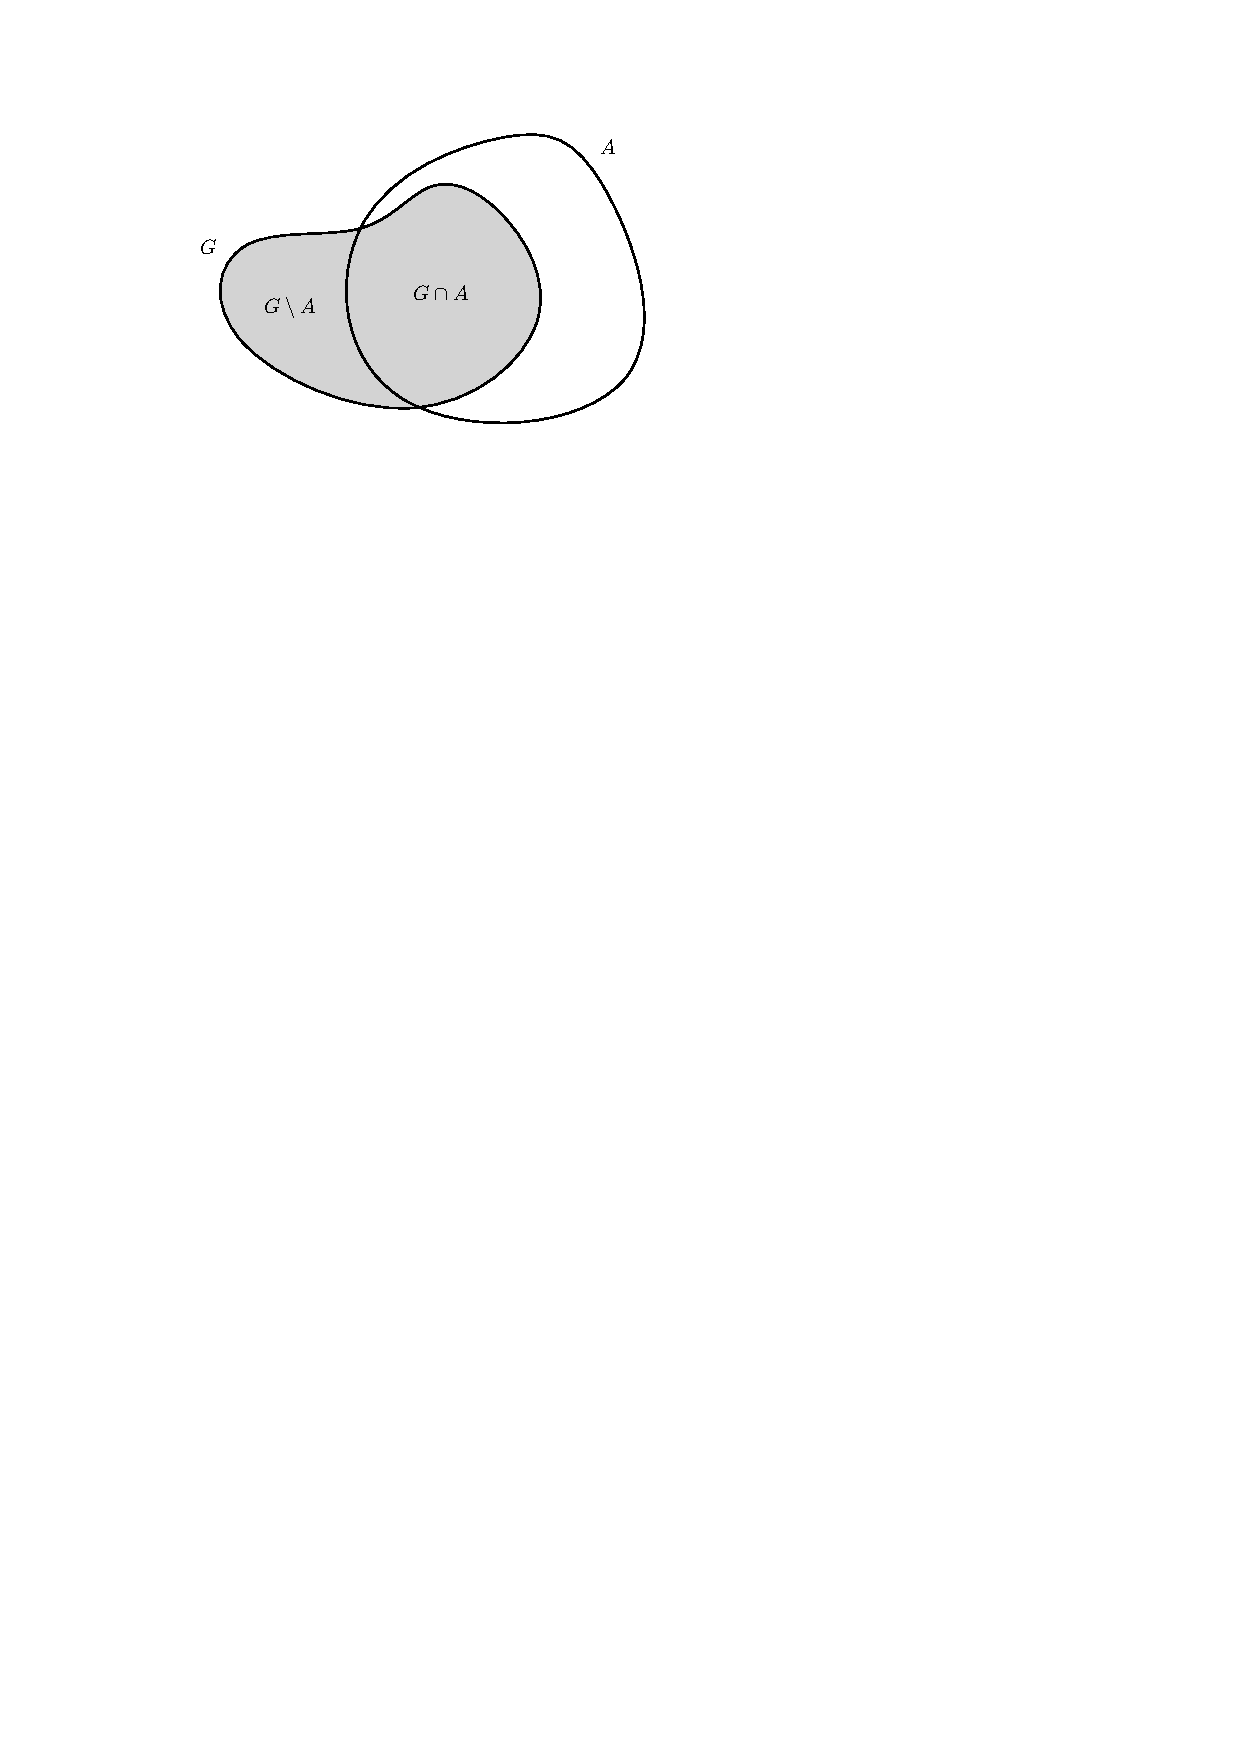
\includegraphics{ch02-caratheodoryho-kriterium.pdf}
    \caption{Ilustrace měřitelnosti množiny $A$}
    \label{fig:caratheodoryho-kriterium}
\end{figure}
O systému $\mathcal{L}(\R^n)$ a Lebesgueově míře $\lambda_n$ lze dokázat následující tvrzení.
\begin{theorem}\label{thm:prostor-s-Lebesgueovou-mirou}
    Platí:
    \begin{enumerate}[label=(\roman*)]
        \item $(\R^n,\mathcal{L}(\R^n))$ je měřitelný prostor.
        \item $(\R^n,\mathcal{L}(\R^n),\lambda_n)$ je prostor s~mírou.
    \end{enumerate}
\end{theorem}
Čtenář snad promine,~že formální důkaz v~případě tohoto tvrzení v~zájmu zachování stručnosti textu zcela vynecháme,~nicméně "zvídavec" jej může nalézt např. v~knize \citep[str. 347]{Royden2010},~kde jsou příslušné záležitosti rozepsány.